% ================================================================
\section{Point-process background}
\label{app:pp}
% ================================================================

This appendix is a self-contained introduction to the point processes used in
Section~\ref{sec:hawkes}: the Poisson, renewal and Hawkes processes, the conditional intensity,
the branching ratio, the Fano factor and the Hurst exponent, and how a Hawkes process is fitted to
data. It assumes no prior knowledge of point processes. It is adapted from Appendix~A of
\citet{maciejewski2026packets}, which also supplies the empirical figures quoted below for CME NQ
market data. Readers who know what a conditional intensity is can go straight to
Section~\ref{app:pp-canon}.

Symbols follow the rest of this paper. For a single event type ($K = 1$) the branching matrix
$\Gamma$ of Section~\ref{sec:hawkes} is a single number, the branching ratio, written $\Gamma$ here
as well. Arrivals are indexed by $n$, as book events are elsewhere in the paper, and a counting
window has length $w$, as the order-flow-imbalance window does.

\subsection{The Poisson process}
\label{app:pp-poisson}

\paragraph{The setup.} Watch packets arrive from a market-data feed and write down the time of
each arrival:
\begin{verbatim}
09:30:00.213    <- 1st arrival
09:30:00.451    <- 2nd
09:30:00.802    <- 3rd
09:30:01.014    <- 4th
09:30:01.317    <- 5th
...
\end{verbatim}
That list of timestamps is the object being modelled. Nothing else---no prices, no sides, only
\emph{when}.

\paragraph{The Poisson idea.} Suppose that in every very small slice of time there is a small,
\emph{independent} chance of an arrival. Independent means that whether an arrival happens now does
not depend on when the previous one came, on how many came in the last minute, or on anything else
about the past. The \emph{rate} of the process is a single number $\mu$, in arrivals per second. At a
rate of $300$ per second, on average $300$ arrivals occur in each second. Three consequences follow
from the independence.

\paragraph{(1) The gap between consecutive arrivals is exponentially distributed with mean
$1/\mu$.} At $\mu = 300$ per second the mean gap is
\[
  \text{mean gap} = \frac{1}{\mu} = \frac{1}{300/\mathrm{s}} \approx 3.3\ \mathrm{ms}.
\]
The gap distribution is \emph{memoryless}: however long one has been waiting, the expected time to
the next arrival is still $3.3$\,ms. The probability that a gap exceeds a length $u$ is
\[
  \P(\text{gap} > u) = \mathrm{e}^{-\mu u},
\]
so at this rate $\P(\text{gap} > 3.3\,\mathrm{ms}) \approx 36.8\%$,
$\P(\text{gap} > 6.6\,\mathrm{ms}) \approx 13.5\%$ and $\P(\text{gap} > 10\,\mathrm{ms}) \approx 5.0\%$.
The probability that a gap is shorter than a tenth of the mean is
\[
  \P\big(\text{gap} < \tfrac{1}{10}\,\text{mean}\big) = 1 - \mathrm{e}^{-0.1} \approx 9.52\%,
\]
whatever the rate. On CME NQ packet data the share is $73\%$~\citep{maciejewski2026packets}.

\begin{figure}[ht]
  \centering
  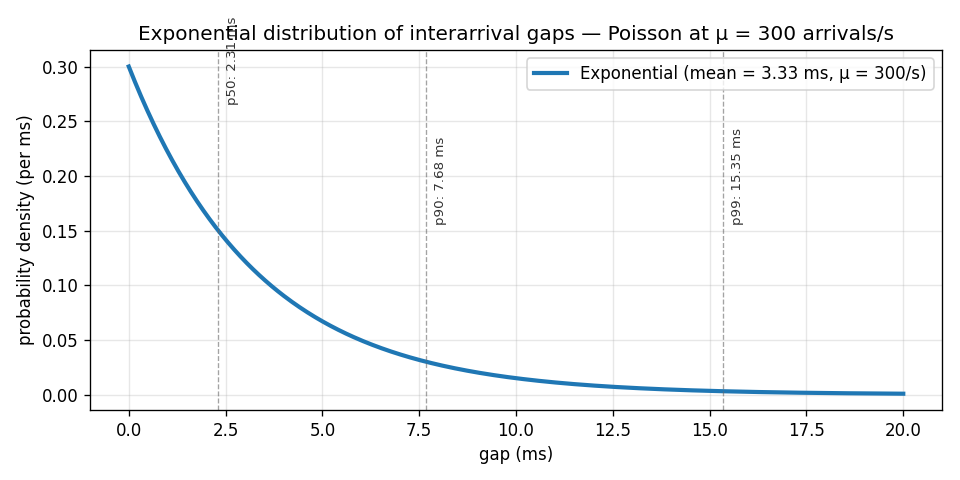
\includegraphics[width=0.7\textwidth]{figs/exponential_gaps.png}
  \caption{The exponential density of the gaps between arrivals of a Poisson process at $300$
  arrivals per second. Dashed vertical lines mark the median, the 90th and the 99th percentile.
  Half the gaps are shorter than the median of $2.3$\,ms and $10\%$ are longer than $7.7$\,ms. Real
  market-data streams have far more mass near zero and a much heavier right tail. Reproduced from
  \citet{maciejewski2026packets}.}
  \label{fig:exp-gaps}
\end{figure}

\paragraph{(2) The count in any window of length $w$ is Poisson-distributed.} Let $N_w$ be the
number of arrivals in a window of length $w$. Then
\[
  \E[N_w] = \mu w, \qquad \mathrm{Var}[N_w] = \mu w,
\]
so the ratio of variance to mean is $1$ for every $w$. This ratio is the \emph{Fano factor}
(Section~\ref{app:pp-fano}); a value other than $1$ rejects the Poisson model.

\paragraph{(3) Counts in non-overlapping windows are independent.} The number of arrivals in the
first second says nothing about the number in the next.

\paragraph{Poisson as the null hypothesis.} The Poisson process is the stream with no memory, no
clustering and no regularity: arrivals are as uncoordinated as possible. Any departure from it is
structure in the arrival stream.

\paragraph{Two ways a real feed departs from Poisson.} The first is \emph{bunching}: many gaps are
far shorter than the exponential law predicts ($73\%$ against $9.52\%$ above). The second is
\emph{memory in the rate}: after a burst starts, more arrivals are likely to follow. Modelling either
needs a process whose rate can change with its own history---a \emph{conditional-intensity point
process}.

\subsection{Points, processes and marks}
\label{app:pp-points}

\begin{itemize}[leftmargin=1.5em,itemsep=1pt]
\item A \textbf{point} is a single instant at which something happens, such as the timestamp of one
  packet or one order-book event.
\item A \textbf{process} is a random object that unfolds in time; here, a random list of arrival
  times $t_1 < t_2 < t_3 < \cdots$.
\item A \textbf{point process} is a random sequence of points on the time axis, specified by
  \emph{when} events happen and nothing else.
\end{itemize}
If each event carries additional information (side, price, size, message type), the process is a
\textbf{marked point process}: the timestamps are the points and the extra information is the
\emph{mark}. Four order-book messages in the first second of a session might read
\begin{verbatim}
09:30:00.001234567   Add,    bid 21432.50, size 3
09:30:00.001234571   Add,    ask 21432.75, size 5
09:30:00.017891234   Cancel, order X, bid 21432.25
09:30:00.238491702   Trade,  ask 21432.75, size 2
\end{verbatim}
The point process is the four timestamps; message type, side, price and size are marks. The
multivariate Hawkes process of Section~\ref{sec:hawkes} is a marked point process whose mark is the
event type $i$.

\subsection{The probability space}
\label{app:pp-probspace}

An arrival stream is modelled as a \textbf{stochastic process}, a family of random variables indexed
by time, on a probability space $(\Omega, \mathcal{A}, \P)$:
\begin{itemize}[leftmargin=1.5em,itemsep=1pt]
\item $\Omega$, the \emph{sample space}, is the set of all possible outcomes; here an outcome is one
  complete realisation of a session's arrivals.
\item $\mathcal{A}$, the \emph{$\sigma$-algebra}, is the collection of yes-or-no questions about the
  outcome to which a probability can be assigned, such as ``did at least one packet arrive between
  09:30:00 and 09:30:01?''. It is closed under negation and countable union.
\item $\P : \mathcal{A} \to [0, 1]$ assigns a probability to each such event, with
  $\P(\emptyset) = 0$, $\P(\Omega) = 1$, and probabilities of disjoint events adding up.
\end{itemize}

\subsection{History: information accumulated over time}
\label{app:pp-history}

The information available at time $t$ grows as time passes. Formally it is a
\textbf{filtration}, an increasing family of $\sigma$-algebras
\[
  \{\mathcal{I}_t\}_{t \ge 0}, \qquad \mathcal{I}_{t'} \subseteq \mathcal{I}_t \text{ for } t' \le t.
\]
$\mathcal{I}_t$ is everything observable up to and including time $t$, and $\mathcal{I}_{t-}$
everything observable strictly before $t$. ``Conditional on $\mathcal{I}_{t-}$'' means ``given
everything seen strictly before $t$''. In the main text this is what conditioning on $X_t$ means: a
model may use only what is in the history.

\subsection{The counting process}
\label{app:pp-counting}

The observable object is the random step function
\[
  N(t) = \#\{\, n : t_n \le t \,\},
\]
the number of arrivals up to time $t$. It starts at $N(0) = 0$, never decreases, and jumps by one at
each arrival. The number of arrivals in the interval $(t, t + \Delta t]$ is $N(t + \Delta t) - N(t)$.

\subsection{Conditional intensity}
\label{app:pp-intensity}

At time $t$, ask for the probability that at least one arrival occurs in the next short interval of
length $\Delta t$, given everything seen so far. The \textbf{conditional intensity} is that
probability divided by $\Delta t$, in the limit of a very short interval:
\[
  \lambda(t \mid \mathcal{I}_{t-}) = \lim_{\Delta t \downarrow 0} \frac{1}{\Delta t}\;
  \P\big( N(t + \Delta t) - N(t) \ge 1 \,\big|\, \mathcal{I}_{t-} \big).
\]
It is the instantaneous arrival rate given the history, in arrivals per second; in the rest of the
paper it is written simply $\lambda(t)$. At an intensity of $300$ per second the probability of an
arrival in the next millisecond is about $\lambda(t)\,\Delta t = 300 \times 0.001 = 0.3$. For a short
interval, and for the expected count over a longer one,
\[
  \P\big(\text{arrival in } (t, t+\Delta t]\big) \approx \lambda(t)\, \Delta t, \qquad
  \E\big[N(t+w) - N(t)\big] = \E\!\int_{t}^{t+w} \lambda(t')\, dt'.
\]
Specifying $\lambda$ as a function of the history specifies the point process completely. For a
Poisson process $\lambda(t) = \mu$ and the history carries no information. For a Hawkes process the
intensity is $\mu$ plus a decaying contribution from each past arrival.

\subsection{Three canonical models: Poisson, renewal and Hawkes}
\label{app:pp-canon}

\paragraph{(a) Poisson.} $\lambda(t) = \mu > 0$. Gaps are independent and exponential with mean
$1/\mu$; the count in a window of length $w$ is Poisson with mean $\mu w$. Every summary statistic
takes its reference value: the Fano factor is $1$ at every $w$, the Hurst exponent is $0.5$, and the
gaps are uncorrelated.

\paragraph{(b) Renewal process.} The gaps $\Delta t_n = t_n - t_{n-1}$ are independent draws from a common
distribution, not necessarily exponential. The intensity depends only on the time since the last
arrival. A renewal process is Poisson only when the gaps are exponential. Heavy-tailed gaps produce
many short gaps and a Fano factor well above $1$, but the Fano factor levels off as $w$ grows instead
of continuing to rise, and the gaps are uncorrelated. Randomly shuffling the order of the gaps leaves
a renewal process statistically unchanged; comparing a statistic on a real stream with the same
statistic on its shuffled gaps therefore separates what the \emph{order} of the gaps carries from
what their \emph{lengths} carry.

\paragraph{(c) Hawkes (self-exciting) process.} Each past arrival raises the intensity for a while:
\[
  \lambda(t) = \mu + \sum_{n:\, t_n < t} \phi(t - t_n).
\]
$\mu \ge 0$ is the \textbf{background rate}, the intensity with no prior arrivals.
$\phi$ is the \textbf{kernel}: an arrival $u$ seconds ago still contributes $\phi(u)$ to the
intensity now. The kernel is the shape of one event's influence on the future. Dropping several
stones into a pond is the usual picture: the disturbance at any moment is the sum of the ripples
still spreading, each faded by the time since its stone fell. For the self-exciting specification
used here the kernel is non-negative, so a past event can only raise future intensity (inhibitory
extensions are discussed in Section~\ref{sec:hawkes-variants}), and its total area
must be finite, so that the past does not accumulate without bound. This is the one-type case of
the multivariate model in Section~\ref{sec:hawkes}.

\paragraph{Kernel families.} The \emph{exponential kernel} $\phi(u) = \alpha\, \mathrm{e}^{-\omega u}$ has
two parameters: $\alpha \ge 0$, the jump in intensity immediately after an arrival, and
$\omega > 0$, the decay rate, whose inverse $1/\omega$ is the kernel's decay time. It is Markovian:
the current intensity summarises everything needed from the past. Right after an arrival the
intensity rises by $\alpha$; between arrivals it relaxes toward $\mu$ as
$\mu + (\lambda(t_n) - \mu)\, \mathrm{e}^{-\omega u}$; so it can be updated in constant time per arrival---a useful
property for a low-latency system. The \emph{power-law kernel} $\phi(u) = \alpha\,(1 + u/u_0)^{-(1+\zeta)}$, with
the same jump $\alpha$, a time scale $u_0 > 0$ and an exponent $\zeta > 0$, decays more slowly; \citet{hardimanbercotbouchaud2013} find power-law kernels on
E-mini S\&P mid-price changes over lags from seconds to days.

\subsection{Branching ratio}
\label{app:pp-branching}

\[
  \Gamma = \int_0^\infty \phi(u)\, du, \qquad \Gamma = \alpha/\omega \text{ for the exponential kernel}.
\]
$\Gamma$ is the mean number of arrivals that one arrival triggers \emph{directly}. The Hawkes process
is equivalently a \textbf{branching process}~\citep{hawkesoakes1974}: every arrival is either an
\emph{immigrant}, generated by the background rate $\mu$, or the \emph{child} of an earlier arrival,
and each arrival has on average $\Gamma$ children. The expected size of the family descended from one
immigrant is the geometric series
\[
  1 + \Gamma + \Gamma^2 + \Gamma^3 + \cdots = \frac{1}{1 - \Gamma} \qquad (\Gamma < 1),
\]
which is the one-type case of the series for $(I - \Gamma)^{-1}$ in Section~\ref{sec:hawkes}. For
$\Gamma < 1$ the process is \emph{subcritical}: families are finite and the long-run rate is
$\bar\lambda = \mu / (1 - \Gamma)$. As $\Gamma \to 1$ it becomes \emph{near-critical}: family sizes
and durations grow without bound and long-range dependence appears. At $\Gamma = 1$ the process is
\emph{critical}: each family still dies out with probability one, but its expected size is infinite,
and with a positive background rate there is no stationary version. For $\Gamma > 1$ it is
\emph{supercritical}: with positive probability one arrival starts a cascade that never ends, and the
intensity grows without bound.

On CME NQ market data, an exponential-kernel fit gives $\Gamma \approx 0.80$ on both packets and
matching-engine transactions, with a kernel decay time $1/\omega$ of about $167\,\mu$s: four of every
five arrivals are triggered by earlier ones~\citep{maciejewski2026packets}.
On E-mini S\&P futures, \citet{filimonovsornette2012} report $0.7$--$0.8$ after 2007, with spikes
to $0.9$, and \citet{hardimanbercotbouchaud2013} report values near $1$ for mid-price changes; \citet{filimonovsornette2015} show that a fit with a
constant background rate, over a window in which the true background varies, overstates $\Gamma$.

\paragraph{The critical boundary in practice.} At $\Gamma = 1$ the stationary rate
$\mu/(1-\Gamma)$ is infinite. On a finite window the process still fires finitely often, but the
variance of the count grows faster than linearly with the window. A maximum-likelihood fit that
lands at $\Gamma = 1$ on real data may signal non-stationarity, a mis-specified kernel or a numerical
problem rather than a genuinely critical market; whether markets are critical or merely close to it is
itself debated~\citep{hardimanbercotbouchaud2013,filimonovsornette2015}.

\subsection{What Hawkes processes look like}
\label{app:pp-visualise}

The long-run rate $\bar\lambda = \mu/(1-\Gamma)$ and the branching ratio $\Gamma$ look different in
an event raster. Figure~\ref{fig:hawkes-grid} simulates an exponential-kernel Hawkes process over
15 seconds at nine combinations, $\bar\lambda \in \{2, 10, 50\}$ events per second and
$\Gamma \in \{0.30, 0.60, 0.90\}$, with a kernel decay time of one second. At low rate and low
branching ratio the stream is nearly Poisson: arrivals spread evenly, the count grows in a straight
line, the intensity is flat. At high rate and low branching ratio it is dense but still nearly
Poisson. At low rate and high branching ratio the mean is 2 per second but arrivals come in
unmistakable bursts, with long empty stretches between them and the intensity reaching 20--30 per
second inside a burst. At high rate and high branching ratio the intensity swings by an order of
magnitude within the window.

\begin{figure}[ht]
  \centering
  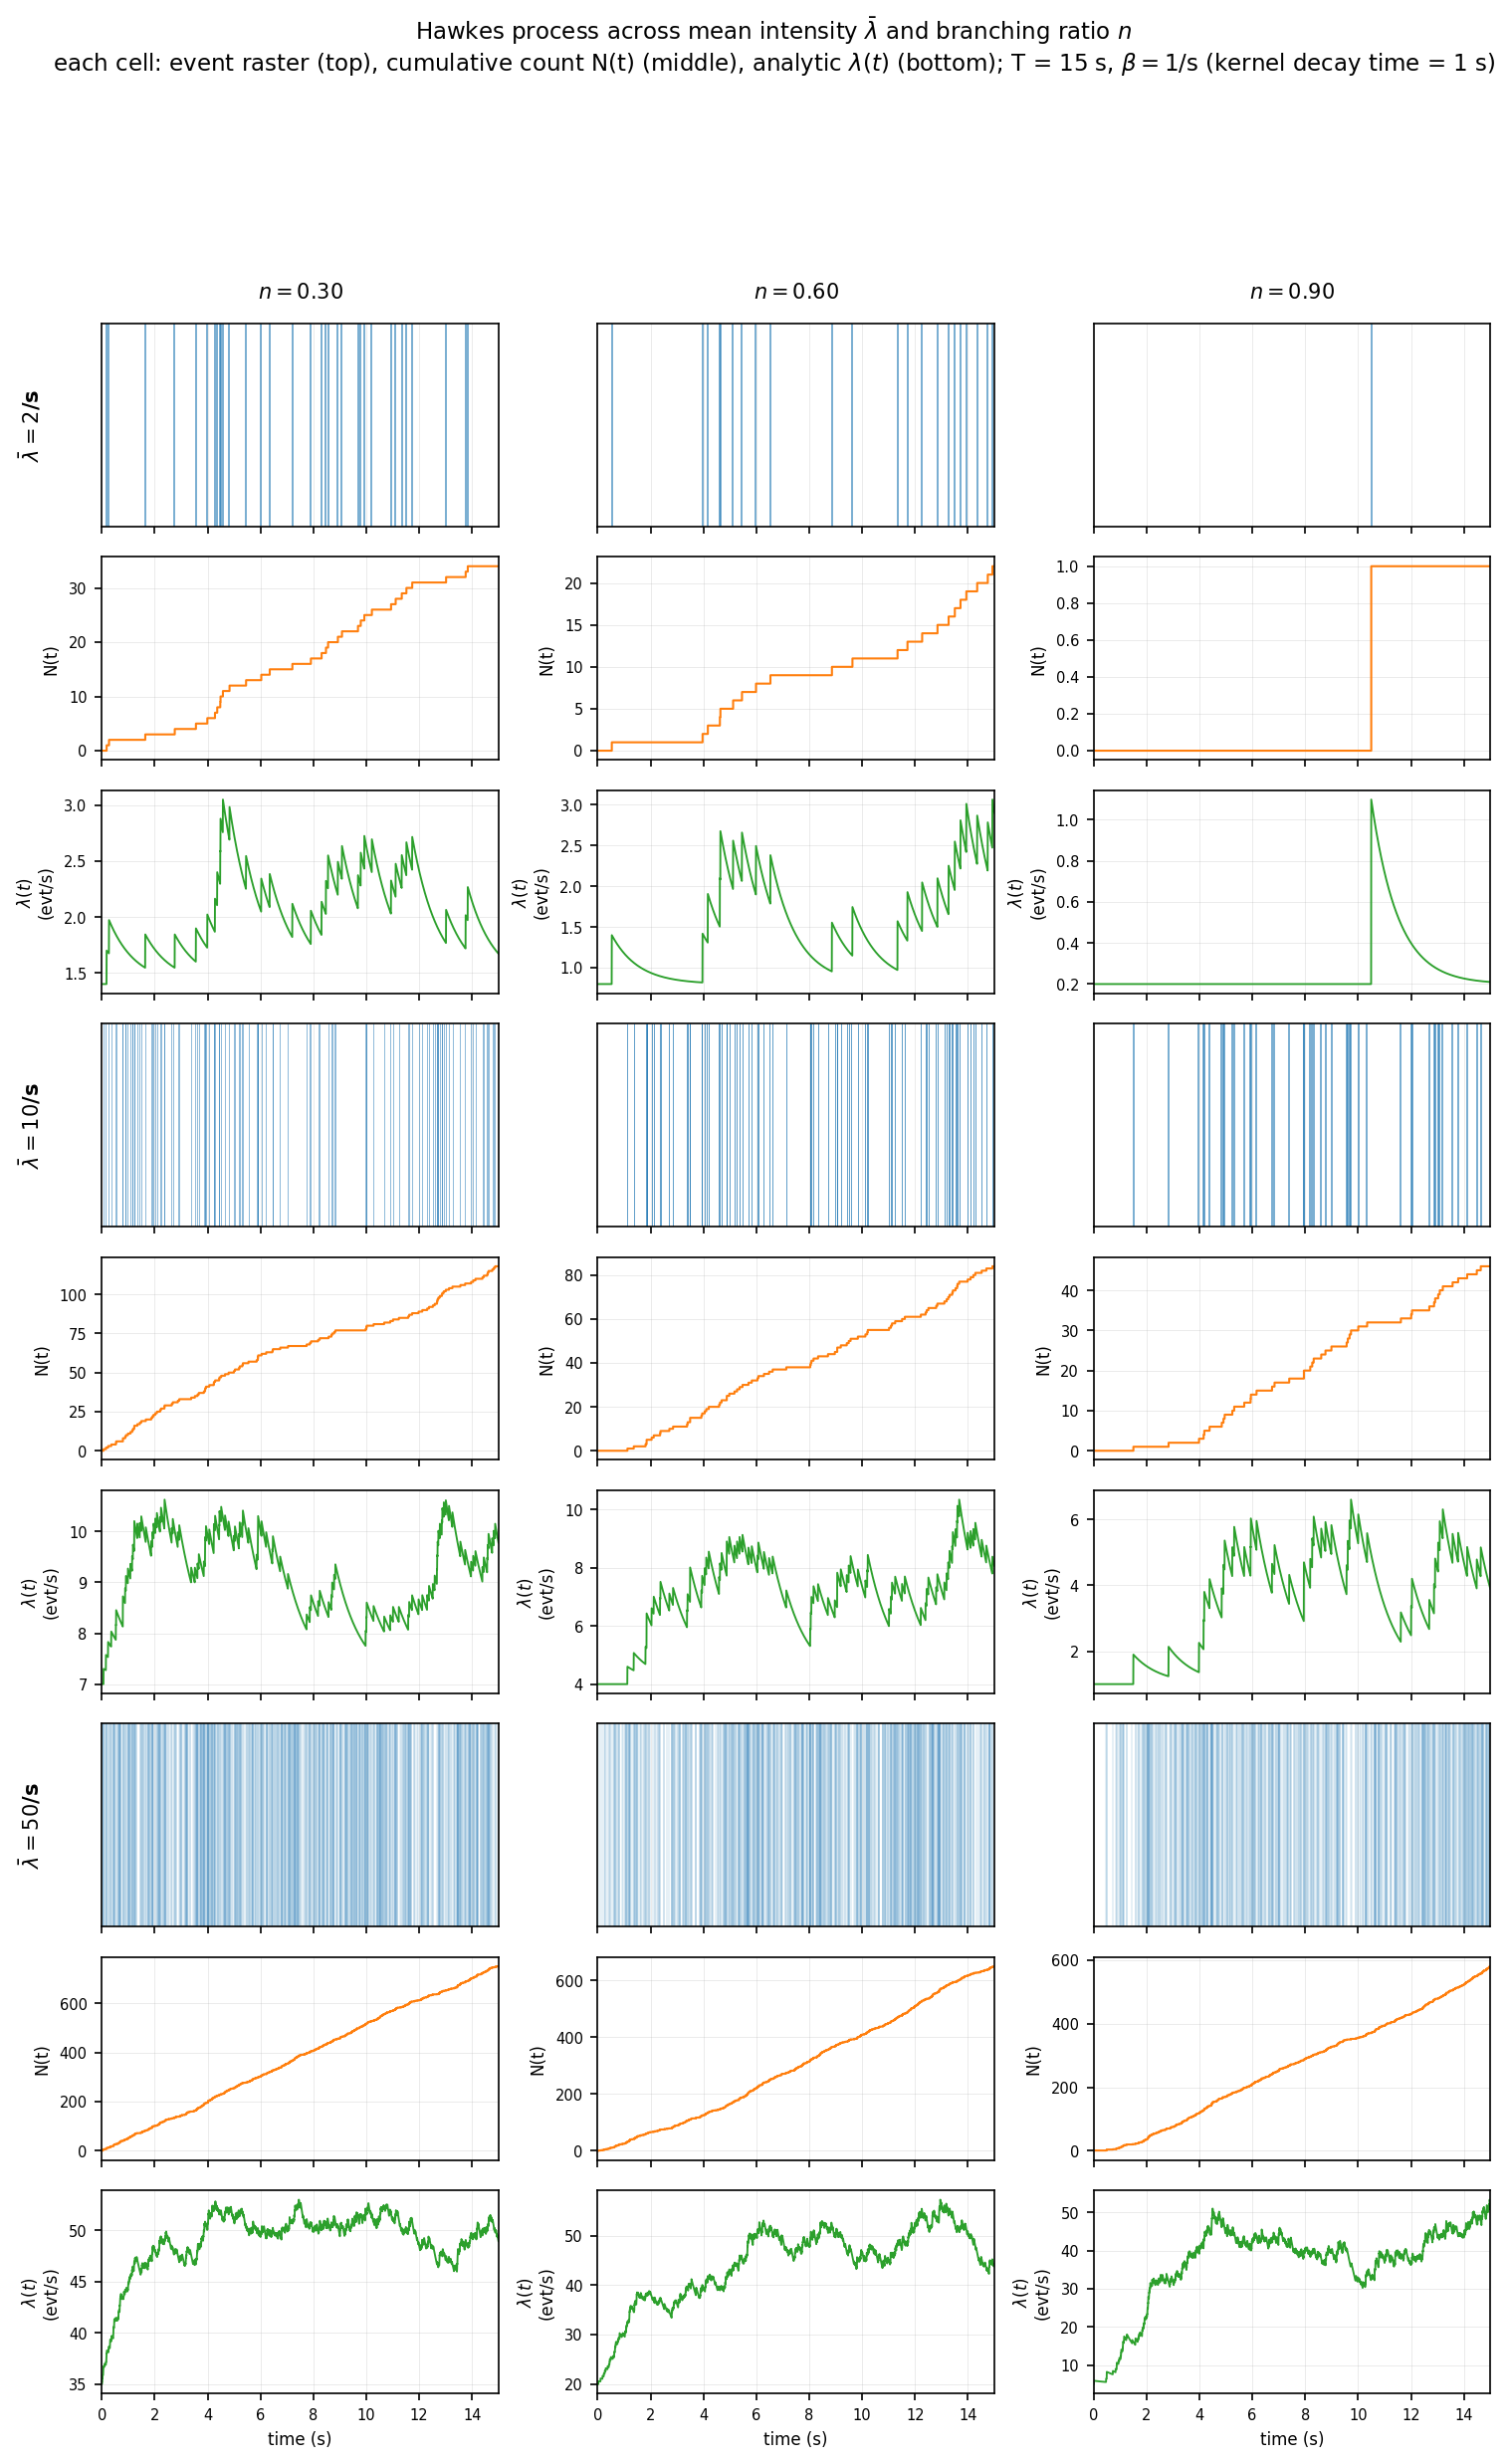
\includegraphics[width=\textwidth,height=0.82\textheight,keepaspectratio]{figs/hawkes_grid_3x3.png}
  \caption{Simulated exponential-kernel Hawkes processes. Each cell stacks the event raster (top),
  the cumulative count $N(t)$ (middle) and the intensity $\lambda(t)$ (bottom). Rows: long-run rate
  $\bar\lambda \in \{2, 10, 50\}$ events per second. Columns: branching ratio
  $\Gamma \in \{0.30, 0.60, 0.90\}$. Fifteen seconds, decay rate $\omega = 1/\mathrm{s}$. The time
  scale is chosen for legibility; the kernel fitted on CME data decays about four orders of
  magnitude faster. Reproduced from \citet{maciejewski2026packets}. Labels inside the image use the source's notation: $n$ for $\Gamma$, $\beta$ for $\omega$, $F$ for $D$ and $\tau$ for $w$.}
  \label{fig:hawkes-grid}
\end{figure}

\subsection{Three signatures that separate Poisson, renewal and Hawkes processes}
\label{app:pp-signatures}

\emph{(i) An excess of short gaps.} On CME NQ packet data $73\%$ of gaps are shorter than a tenth of
the mean gap; any exponential gives $9.52\%$. A Hawkes process produces such an excess, but so does a
renewal process with heavy-tailed gaps, so this signature rejects Poisson without identifying
self-excitation.

\emph{(ii) Correlated gaps.} Under self-excitation, short gaps tend to follow short gaps and long
gaps follow long ones, so successive gaps are positively correlated. A renewal process has
independent gaps. A rate that varies slowly over the observation window also produces positive gap
correlation, so this signature has to be checked against that alternative.

\emph{(iii) Burstiness that grows with the time scale.} The Fano factor rises with the window length
on a Hawkes process and levels off on a Poisson or renewal process. Clustering is then not a feature
of one time scale but looks similar over decades of window lengths. A slowly varying rate can also
make the Fano factor rise, which is the effect \citet{filimonovsornette2015} warn about.

\subsection{Fano factor}
\label{app:pp-fano}

For a window length $w$, cut the observation period into $\Upsilon$ consecutive windows and let
$N_{w,\upsilon} = N(\upsilon w) - N((\upsilon-1)w)$ be the count in window $\upsilon$. The Fano factor, also called the
\emph{index of dispersion}, is
\[
  D(w) = \frac{\mathrm{Var}[N_{w,\upsilon}]}{\E[N_{w,\upsilon}]},
\]
the variance of the window counts divided by their mean. For a Poisson process $D(w) = 1$ at every
$w$. For a renewal process with finite-variance gaps $D(w)$ tends to a constant as $w$ grows. For a
clustered process $D(w) > 1$, and under self-excitation or a varying rate it keeps growing with $w$.
The measure is named after U.~Fano, who introduced it for fluctuations in counts of ions. On CME NQ
packet data $D(w)$ grows from about $52$ at $w = 0.1$\,s to about a thousand at $w = 60$\,s, while
the same stream with its gaps shuffled stays flat at about $17$~\citep{maciejewski2026packets}.

\begin{figure}[ht]
  \centering
  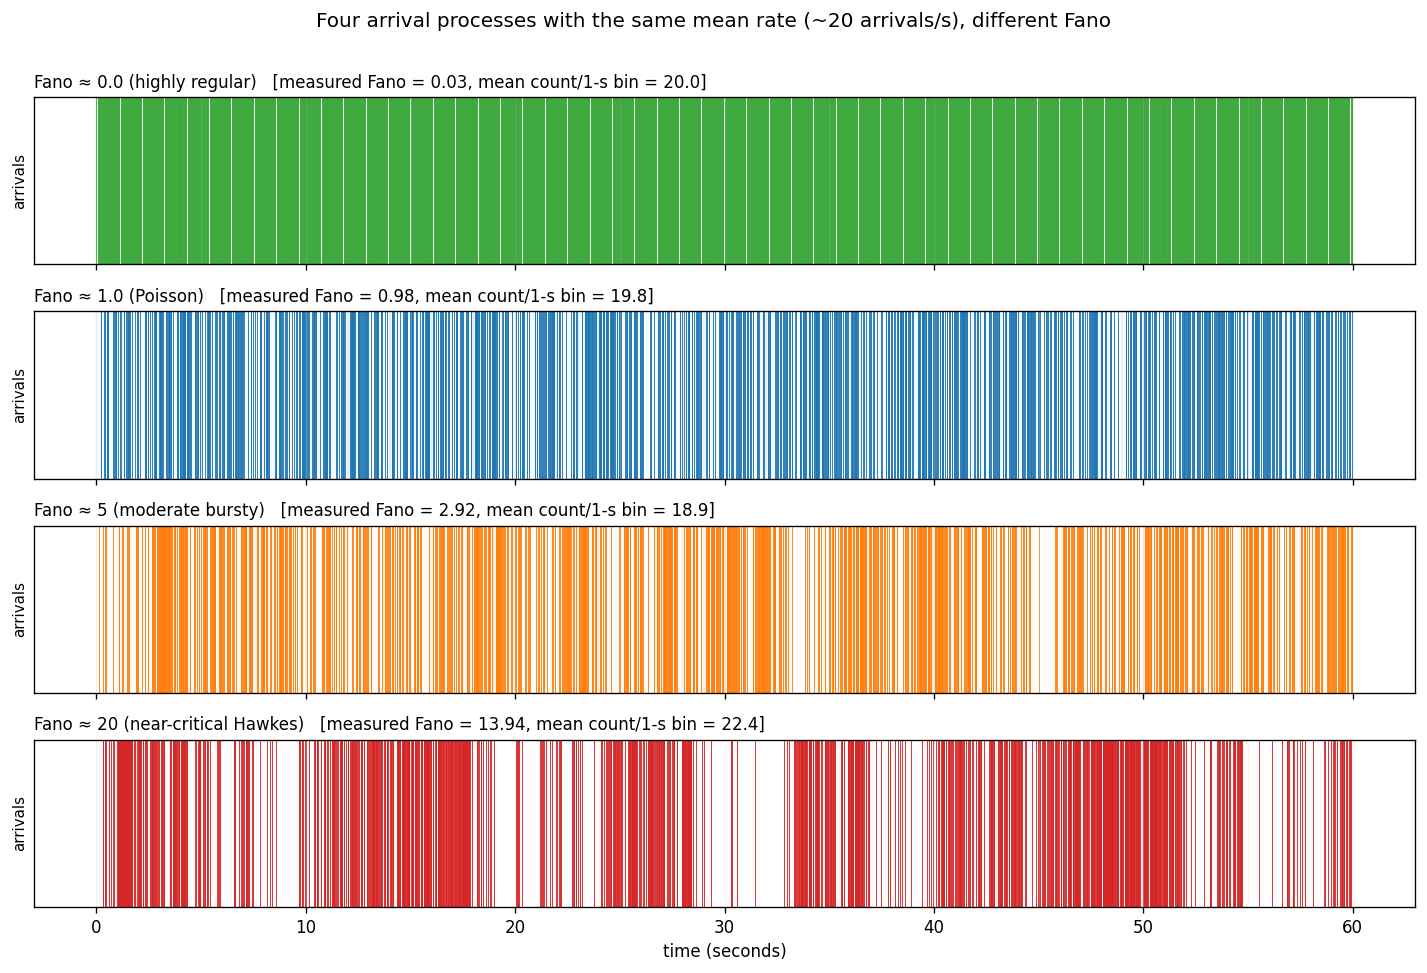
\includegraphics[width=\textwidth]{figs/rasters_by_fano.png}
  \caption{Four simulated processes at the same mean rate of about 20 per second. Top row
  ($D \approx 0$, highly regular): near-lattice arrivals, nearly equal counts per window. Second row
  ($D \approx 1$, Poisson): the reference. Third row ($D \approx 3$, moderate Hawkes): visible
  clumping. Bottom row ($D \approx 14$, near-critical Hawkes): pronounced bursts and long quiet
  stretches, with window counts from near zero to over 50. Reproduced from
  \citet{maciejewski2026packets}. Labels inside the image use the source's notation: $n$ for $\Gamma$, $\beta$ for $\omega$, $F$ for $D$ and $\tau$ for $w$.}
  \label{fig:rasters-fano}
\end{figure}

\begin{figure}[ht]
  \centering
  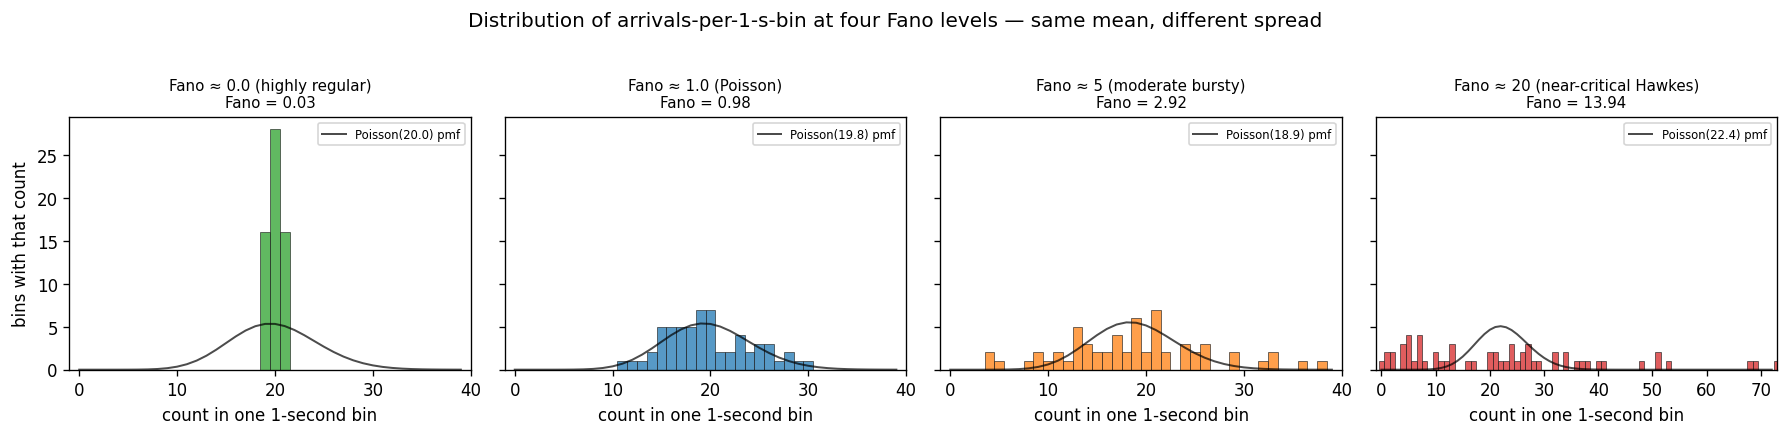
\includegraphics[width=\textwidth]{figs/count_hists_by_fano.png}
  \caption{Distribution of arrivals per one-second window (bars) for the four processes of
  Figure~\ref{fig:rasters-fano}, with the Poisson distribution of the same mean overlaid (curve).
  $D \approx 0$: narrower than Poisson. $D \approx 1$: matches Poisson. $D > 1$: wider than Poisson,
  with extra mass in both tails. The CME NQ packet stream has $D(1\,\mathrm{s}) = 108$, far wider
  than any panel shown. Reproduced from \citet{maciejewski2026packets}. Labels inside the image use the source's notation: $n$ for $\Gamma$, $\beta$ for $\omega$, $F$ for $D$ and $\tau$ for $w$.}
  \label{fig:counthist-fano}
\end{figure}

\subsection{Hurst exponent from the scaling of the Fano factor}
\label{app:pp-hurst}

When the Fano factor grows as a power of the window length,
\[
  D(w) \propto w^{2\mathcal{H} - 1},
\]
the exponent $\mathcal{H}$ is the \emph{Hurst exponent}. $\mathcal{H} = 0.5$ means no long-range
dependence (Poisson, and renewal processes with finite-variance gaps); $0.5 < \mathcal{H} < 1$ means
long-range dependence, with clustering that looks similar across time scales; $\mathcal{H}$ near $1$
means very long memory. It is estimated by a straight-line fit on a log--log plot,
\[
  \ln D(w) = (2\mathcal{H} - 1)\ln w + \text{constant},
\]
so $\mathcal{H} = (\text{slope} + 1)/2$. On CME NQ packet data $\mathcal{H} \approx 0.74$; shuffling
the gaps, which keeps their lengths and destroys their order, takes it to $0.50$, so the long-range
dependence lives in the order of the gaps~\citep{maciejewski2026packets}.

\begin{figure}[ht]
  \centering
  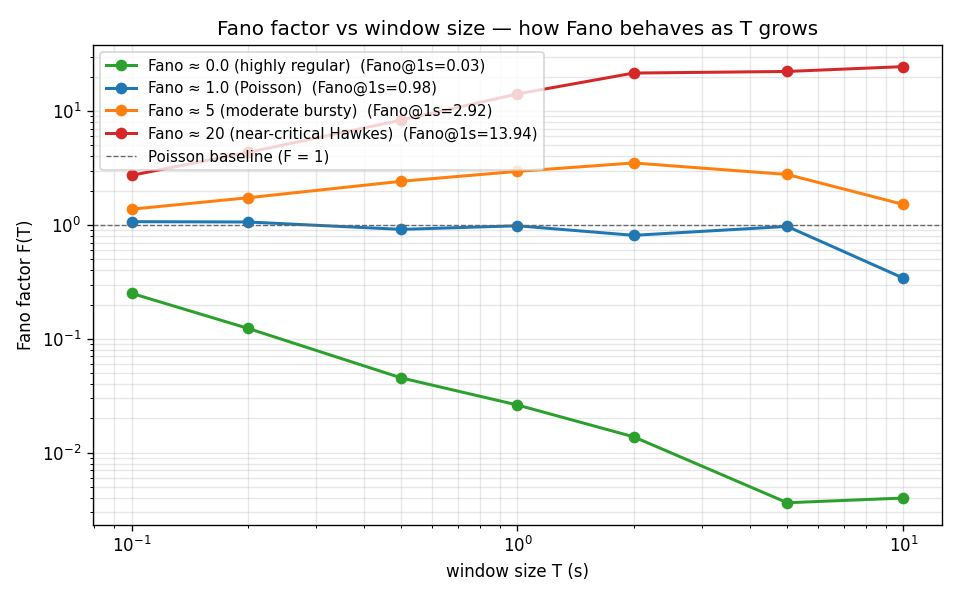
\includegraphics[width=0.7\textwidth]{figs/fano_scaling.png}
  \caption{The Fano factor $D(w)$ against the window length $w$ on logarithmic axes for four
  simulated processes. Regular: near zero. Poisson: flat at 1. Moderate Hawkes: rising. Near-critical
  Hawkes: a steeper rise, with slope about $0.5$, i.e.\ $\mathcal{H} \approx 0.75$. Reproduced from
  \citet{maciejewski2026packets}. Labels inside the image use the source's notation: $n$ for $\Gamma$, $\beta$ for $\omega$, $F$ for $D$ and $\tau$ for $w$.}
  \label{fig:fano-scaling}
\end{figure}

\subsection{Fitting an exponential-kernel Hawkes process}
\label{app:pp-mle}

The input is a sorted list of arrival times $t_1 < \cdots < t_{N_{\text{end}}}$ in a window
$[0, t_{\text{end}}]$, where $N_{\text{end}} = N(t_{\text{end}})$ is the number of arrivals, and
there are three parameters:
\begin{itemize}[leftmargin=1.5em,itemsep=1pt]
\item $\mu$, the \textbf{background rate}: arrivals per second with no recent history;
\item $\alpha$, the \textbf{jump}: the rise in intensity, in arrivals per second, at each arrival;
\item $\omega$, the \textbf{decay rate}: each jump fades as $\mathrm{e}^{-\omega u}$, with decay time
  $1/\omega$.
\end{itemize}
Fitting means choosing the parameters under which the observed timestamps are most probable, that
is, maximising the log-likelihood~\citep{ozaki1979}
\begin{equation}
  \ln \mathrm{Lik}(\mu, \alpha, \omega) = \sum_{n=1}^{N_{\text{end}}} \ln \lambda(t_n)
  - \int_0^{t_{\text{end}}} \lambda(t')\, dt'.
  \label{eq:hawkes-loglik}
\end{equation}
\inwords{the first term rewards the model for predicting a high rate at the moments arrivals
actually happened; the second penalises it for predicting more arrivals in total than occurred. If
$\alpha$ is too small the model cannot explain the bursts; if $\alpha$ approaches $\omega$ it predicts
more clustering than there is; a wrong $\mu$ misexplains the quiet periods.}

For the exponential kernel both terms can be computed in one pass over the data. With
\[
  \Psi_n = \mathrm{e}^{-\omega (t_n - t_{n-1})}\,(1 + \Psi_{n-1}), \qquad \Psi_1 = 0,
\]
the intensity at each arrival is $\lambda(t_n) = \mu + \alpha \Psi_n$, and the integral is
\[
  \int_0^{t_{\text{end}}} \lambda(t')\, dt' = \mu\, t_{\text{end}}
  + \frac{\alpha}{\omega} \sum_{n=1}^{N_{\text{end}}} \Big(1 - \mathrm{e}^{-\omega (t_{\text{end}} - t_n)}\Big).
\]
Timestamps are shifted to the start of the window before fitting, so that the exponentials do not
underflow. The log-likelihood is then maximised numerically over $(\mu, \alpha, \omega)$, for example
with the Nelder--Mead method, and the optimum checked with a second optimiser. From the fitted
parameters follow the branching ratio $\Gamma = \alpha/\omega$, the kernel decay time $1/\omega$, and
the long-run rate $\bar\lambda = \mu/(1 - \Gamma)$: the background rate amplified by $1/(1-\Gamma)$
through self-excitation.

\subsection{Symbols used in this appendix}

\begin{center}\small
\begin{tabular}{@{}ll@{}}
\toprule
Symbol & Meaning \\
\midrule
$\Omega$, $\mathcal{A}$, $\P$ & sample space, $\sigma$-algebra, probability \\
$\mathcal{I}_t$, $\mathcal{I}_{t-}$ & everything observable up to $t$ inclusive / strictly before $t$ \\
$t_1, t_2, \ldots$ & arrival times \\
$N(t)$ & counting process, the number of arrivals up to $t$ \\
$\lambda(t)$ & conditional intensity, arrivals per second \\
$\mu$ & background rate \\
$\phi(u)$ & Hawkes kernel \\
$\alpha$, $\omega$ & exponential-kernel jump and decay rate; decay time $1/\omega$ \\
$\Gamma$ & branching ratio, $\int\phi$; $\alpha/\omega$ for the exponential kernel \\
$\bar\lambda = \mu/(1-\Gamma)$ & long-run mean rate \\
$\Delta t_n = t_n - t_{n-1}$ & gap between arrivals \\
$w$ & window length for counts \\
$N_{w,\upsilon}$, $\Upsilon$ & arrivals in window $\upsilon$; number of windows \\
$D(w)$ & Fano factor, variance over mean of the window counts \\
$\mathcal{H}$ & Hurst exponent, $D(w) \propto w^{2\mathcal{H}-1}$ \\
$\Psi_n$ & running sum used to compute $\lambda(t_n)$ in one pass \\
\bottomrule
\end{tabular}
\end{center}
